\newpage
\section{Geometry}

\subsection{Formulas for Area and Perimeter of Geometric Figures}

\begin{itemize}
	
	\item \textbf{Square}
	      \begin{itemize}
		      \item Area: \(A = a^2\)
		      \item Perimeter: \(P = 4a\)
	      \end{itemize}

	\item \textbf{Rectangle}
	      \begin{itemize}
		      \item Area: \(A = l \cdot w\)
		      \item Perimeter: \(P = 2(l + w)\)
	      \end{itemize}

	\item \textbf{Circle}
	      \begin{itemize}
		      \item Area: \(A = \pi r^2\)
		      \item Circumference: \(C = 2\pi r\)
	      \end{itemize}

	\item \textbf{Triangle (General)}
	      \begin{itemize}
		      \item Area: \(A = \frac{1}{2} b \cdot h\)
		      \item Perimeter: \(P = a + b + c\)
	      \end{itemize}

	\item \textbf{Equilateral Triangle}
	      \begin{itemize}
		      \item Area: \(A = \frac{\sqrt{3}}{4} a^2\)
		      \item Perimeter: \(P = 3a\)
	      \end{itemize}

	\item \textbf{Isosceles Triangle}
	      \begin{itemize}
		      \item Area: \(A = \frac{b}{4} \sqrt{4a^2 - b^2}\)
	      \end{itemize}

	\item \textbf{Trapezoid}
	      \begin{itemize}
		      \item Area: \(A = \frac{1}{2}(a + b)h\)
		      \item Perimeter: \(P = a + b + c + d\)
	      \end{itemize}

	\item \textbf{Parallelogram}
	      \begin{itemize}
		      \item Area: \(A = b \cdot h\)
		      \item Perimeter: \(P = 2(a + b)\)
	      \end{itemize}

\end{itemize}

\subsection{Formulas for Area and Volume of 3D Geometric Figures}

\begin{itemize}
	\item \textbf{Cube}
	      \begin{itemize}
		      \item Surface Area: \(A = 6a^2\)
		      \item Volume: \(V = a^3\)
	      \end{itemize}

	\item \textbf{Cylinder}
	      \begin{itemize}
		      \item Surface Area: \(A = 2\pi r(h + r)\)
		      \item Volume: \(V = \pi r^2 h\)
	      \end{itemize}

	\item \textbf{Cone}
	      \begin{itemize}
		      \item Surface Area: \(A = \pi r(r + l)\) with \(l\) = slant height
		      \item Volume: \(V = \frac{1}{3}\pi r^2 h\)
	      \end{itemize}

	\item \textbf{Sphere}
	      \begin{itemize}
		      \item Surface Area: \(A = 4\pi r^2\)
		      \item Volume: \(V = \frac{4}{3} \pi r^3\)
	      \end{itemize}

	\item \textbf{Square Pyramid}
	      \begin{itemize}
		      \item Surface Area: \(A = a^2 + 2a \cdot l\)
		      \item Volume: \(V = \frac{1}{3} a^2 h\)
	      \end{itemize}

	\item \textbf{Triangular Pyramid (Tetrahedron)}
	      \begin{itemize}
		      \item Volume: \(V = \frac{1}{3} A_b \cdot h\)
	      \end{itemize}

	\item \textbf{Prism (General)}
	      \begin{itemize}
		      \item Surface Area: \(A = 2A_b + P_b \cdot h\)
		      \item Volume: \(V = A_b \cdot h\)
	      \end{itemize}
\end{itemize}

\subsection{Thales' Theorem}

Thales' Theorem states:
If \(A\), \(B\), and \(c\) are points on a circle where the line \( AB \) is the diameter, 
then the angle \( \angle  \alpha + \beta\) is a right angle.

\begin{align*}
	\angle \alpha + \beta = 90^\circ \quad \text{if } AB \text{ is a diameter of the circle}
\end{align*}

\begin{center}
\begin{tikzpicture}[rotate=36.9,scale=2]
  \tkzDefPoint(0,0){A}
  \tkzDefPoint(4,0){C}
  \tkzDefTriangle[egyptian](A,C) \tkzGetPoint{B}
  \tkzDrawPolygon(A,B,C)
  \tkzDefMidPoint(A,B) \tkzGetPoint{O}
  \tkzDrawSemiCircle(O,B)
  \tkzDrawSegment(O,C)
  \tkzLabelPoints(O,A,B)
  \tkzLabelPoints[above](C)
  \tkzMarkRightAngle[fill=teal!20,opacity=.4](B,C,A)
  \tkzLabelAngles[pos=.75](B,A,C A,C,O){$\alpha$}
  \tkzLabelAngles[pos=.75](C,B,O O,C,B){$\beta$}
   \tkzMarkAngles[mark=|](B,A,C A,C,O)
   \tkzMarkAngles[mark=||](C,B,O O,C,B)
 \end{tikzpicture}
\end{center}

\textbf{Proof:}

Note that we have two Isosceles triangles where the sides \(AO\), \(AC\) and \(OC\) have all the same 
length, being this the radius of the circle.

Because they are Isosceles then two of their angles have to be equal and the sum of the angles 
of this two triangle has to add up to the be \(180^\circ\). Therefore, 

\begin{align*}
	\alpha + \alpha + \beta + \beta &= 180 \\
	2 \alpha + 2\beta &= 180 \\
	\alpha + \beta = 90
\end{align*}

\QED

\subsection{Conversion Between Radians and Degrees}

To convert between radians and degrees, use the following formulas:

\begin{align*}
	\text{Degrees} & = \text{Radians} \times \left( \frac{180^\circ}{\pi} \right) \\
	\text{Radians} & = \text{Degrees} \times \left( \frac{\pi}{180^\circ} \right)
\end{align*}

\subsection{Geometric Figures with Formulas (2D)}

\subsection*{Square and Rectangle}

\begin{center}
	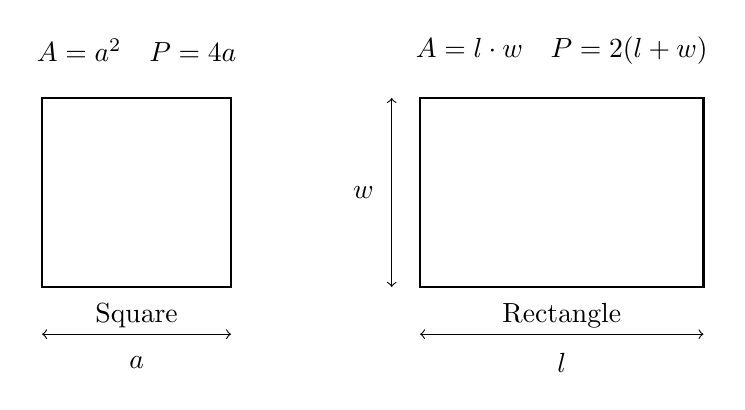
\begin{tikzpicture}[scale=1.2]
		% Square
		\draw[thick] (0,0) rectangle (2,2);
		\node at (1,-0.3) {Square};
		\draw[<->] (0,-0.5) -- (2,-0.5);
		\node at (1,-0.8) {\(a\)};
		\node at (1,2.5) {\(A = a^2 \quad P = 4a\)};

		% Rectangle
		\draw[thick] (4,0) rectangle (7,2);
		\node at (5.5,-0.3) {Rectangle};
		\draw[<->] (4,-0.5) -- (7,-0.5);
		\node at (5.5,-0.8) {\(l\)};
		\draw[<->] (3.7,0) -- (3.7,2);
		\node at (3.4,1) {\(w\)};
		\node at (5.5,2.5) {\(A = l \cdot w \quad P = 2(l+w)\)};
	\end{tikzpicture}
\end{center}

\subsection*{Circle and Triangle Types}

\begin{center}
	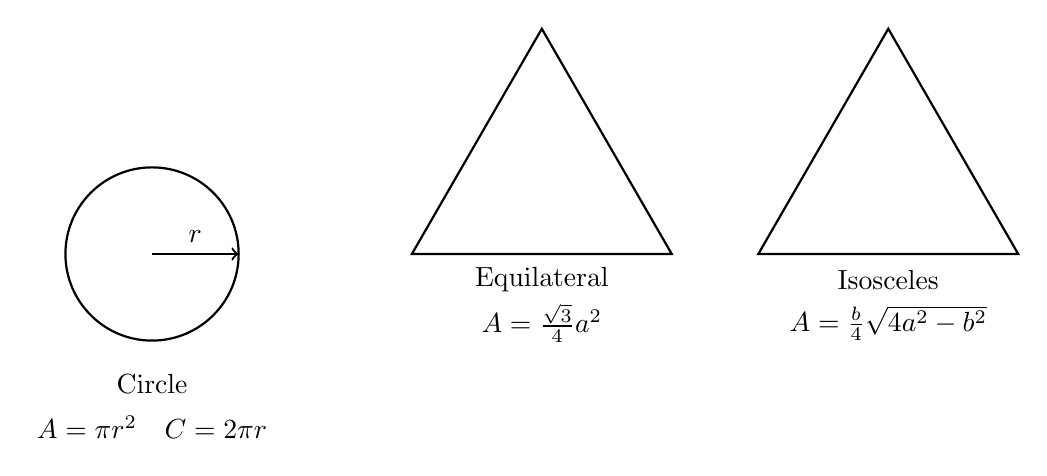
\begin{tikzpicture}[scale=1.1]
		% Circle
		\draw[thick] (0,0) circle(1cm);
		\draw[thick, ->] (0,0) -- (1,0);
		\node at (0.5,0.2) {\(r\)};
		\node at (0,-1.5) {Circle};
		\node at (0,-2) {\(A = \pi r^2 \quad C = 2\pi r\)};

		% Equilateral Triangle
		\draw[thick] (3,0) -- (4.5,2.6) -- (6,0) -- cycle;
		\node at (4.5,-0.3) {Equilateral};
		\node at (4.5,-0.8) {\(A = \frac{\sqrt{3}}{4} a^2\)};

		% Isosceles Triangle
		\draw[thick] (7,0) -- (8.5,2.6) -- (10,0) -- cycle;
		\node at (8.5,-0.3) {Isosceles};
		\node at (8.5,-0.8) {\(A = \frac{b}{4} \sqrt{4a^2 - b^2}\)};
	\end{tikzpicture}
\end{center}

\subsection*{Scalene Triangle, Trapezoid, Parallelogram}

\begin{center}
	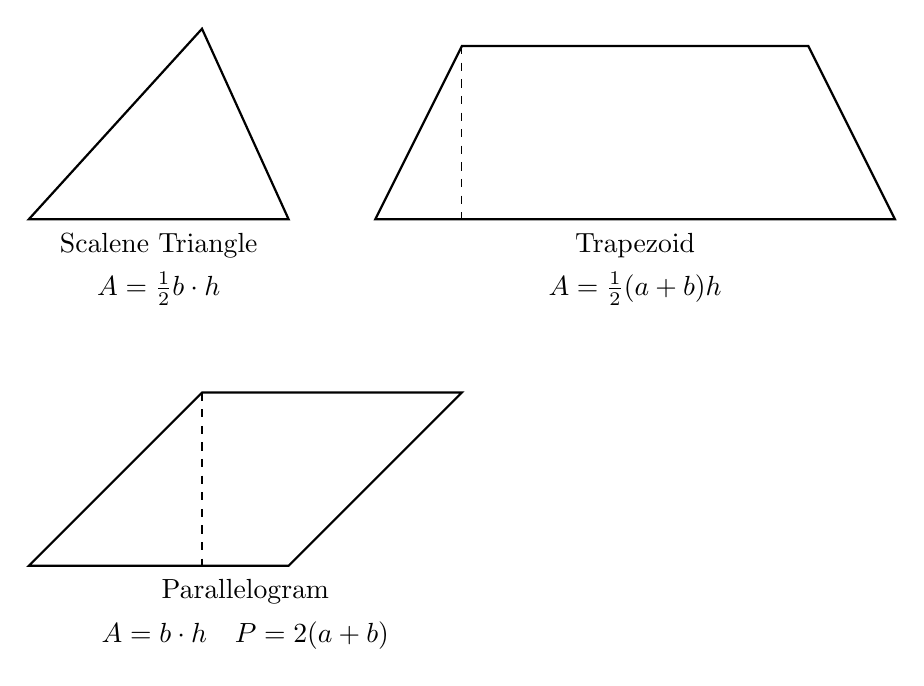
\begin{tikzpicture}[scale=1.1]
		% Scalene Triangle
		\draw[thick] (0,0) -- (2,2.2) -- (3,0) -- cycle;
		\node at (1.5,-0.3) {Scalene Triangle};
		\node at (1.5,-0.8) {\(A = \frac{1}{2} b \cdot h\)};

		% Trapezoid
		\draw[thick] (4,0) -- (5,2) -- (9,2) -- (10,0) -- cycle;
		\draw[dashed] (5,2) -- (5,0);
		\node at (7,-0.3) {Trapezoid};
		\node at (7,-0.8) {\(A = \frac{1}{2}(a+b)h\)};

		% Parallelogram
		\draw[thick] (0,-4) -- (2,-2) -- (5,-2) -- (3,-4) -- cycle;
		\draw[dashed] (2,-2) -- (2,-4);
		\node at (2.5,-4.3) {Parallelogram};
		\node at (2.5,-4.8) {\(A = b \cdot h \quad P = 2(a + b)\)};
	\end{tikzpicture}
\end{center}

\subsection{3D Geometric Figures with Formulas}

\subsubsection{Cube and Cylinder}

\begin{center}
	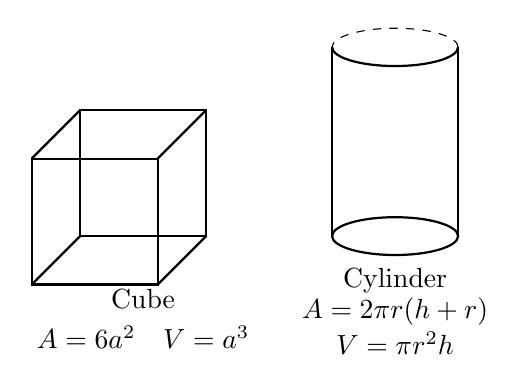
\begin{tikzpicture}[scale=0.8]
		% Cube
		\draw[thick] (0,0,0) -- (2,0,0) -- (2,2,0) -- (0,2,0) -- cycle;
		\draw[thick] (0,0,0) -- (0,0,2);
		\draw[thick] (2,0,0) -- (2,0,2);
		\draw[thick] (2,2,0) -- (2,2,2);
		\draw[thick] (0,2,0) -- (0,2,2);
		\draw[thick] (0,0,2) -- (2,0,2) -- (2,2,2) -- (0,2,2) -- cycle;
		\node at (1,-1) {Cube};
		\node at (1,-1.6) {\(A = 6a^2 \quad V = a^3\)};

		% Cylinder
		\begin{scope}[xshift=5cm]
			\draw[thick] (0,0) ellipse (1 and 0.3);
			\draw[thick] (-1,0) -- (-1,3);
			\draw[thick] (1,0) -- (1,3);
			\draw[thick] (-1,3) arc (180:360:1 and 0.3);
			\draw[dashed] (1,3) arc (0:180:1 and 0.3);
			\node at (0, -0.7) {Cylinder};
			\node at (0, -1.2) {\(A = 2\pi r(h + r)\)};
			\node at (0, -1.7) {\(V = \pi r^2 h\)};
		\end{scope}
	\end{tikzpicture}
\end{center}

\subsubsection{Cone and Sphere}

\begin{center}
	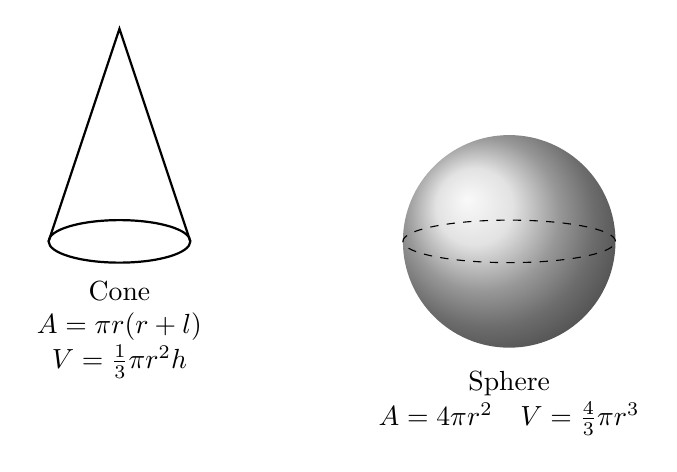
\begin{tikzpicture}[scale=0.9]
		% Cone
		\draw[thick] (0,0) ellipse (1 and 0.3);
		\draw[thick] (-1,0) -- (0,3) -- (1,0);
		\draw[dashed] (1,0) arc (0:180:1 and 0.3);
		\node at (0,-0.7) {Cone};
		\node at (0,-1.2) {\(A = \pi r(r + l)\)};
		\node at (0,-1.7) {\(V = \frac{1}{3} \pi r^2 h\)};

		% Sphere
		\begin{scope}[xshift=5.5cm]
			\shade[ball color=gray!30] (0,0) circle (1.5);
			\draw[dashed] (0,0) ellipse (1.5 and 0.3);
			\node at (0,-2) {Sphere};
			\node at (0,-2.5) {\(A = 4\pi r^2 \quad V = \frac{4}{3} \pi r^3\)};
		\end{scope}
	\end{tikzpicture}
\end{center}

\subsubsection{Pyramid and Prism}

\begin{center}
	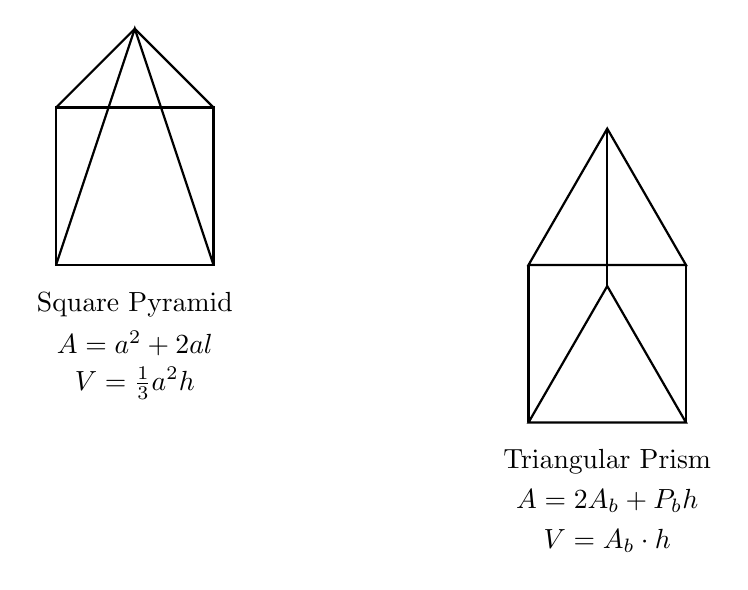
\begin{tikzpicture}[scale=1]
		% Square Pyramid
		\draw[thick] (0,0) -- (2,0) -- (2,2) -- (0,2) -- cycle;
		\draw[thick] (0,0) -- (1,3) -- (2,0);
		\draw[thick] (2,2) -- (1,3) -- (0,2);
		\node at (1,-0.5) {Square Pyramid};
		\node at (1,-1) {\(A = a^2 + 2al\)};
		\node at (1,-1.5) {\(V = \frac{1}{3}a^2 h\)};

		% Triangular Prism
		\begin{scope}[xshift=6cm]
			\draw[thick] (0,0) -- (2,0) -- (1,1.732) -- cycle;
			\draw[thick] (0,0) -- (0,-2);
			\draw[thick] (2,0) -- (2,-2);
			\draw[thick] (1,1.732) -- (1,-0.268);
			\draw[thick] (0,-2) -- (2,-2) -- (1,-0.268) -- cycle;
			\node at (1,-2.5) {Triangular Prism};
			\node at (1,-3) {\(A = 2A_b + P_b h\)};
			\node at (1,-3.5) {\(V = A_b \cdot h\)};
		\end{scope}
	\end{tikzpicture}
\end{center}

\subsection{Axioms of Euclidean Geometry}

Euclidean geometry is founded on a set of basic assumptions known as axioms or postulates, originally 
formulated by the Greek mathematician Euclid in his work \textit{Elements}. These axioms form the logical 
basis for plane geometry and include the following:

\begin{enumerate}[label=\Roman*.]

	\item \emph{Line Postulate:} A straight line segment can be drawn joining any two points.
    
    \item \emph{Extension Postulate:} Any straight line segment can be extended indefinitely in a straight 
			line.
    
    \item \emph{Circle Postulate:} Given any straight line segment, a circle can be drawn having the 
		   segment as radius and one endpoint as center.
    
    \item \emph{Right Angle Postulate:} All right angles are congruent.
    
    \item \emph{Parallel Postulate:} If a line segment intersects two straight lines and makes the interior  
	      angles on the same side less than two right angles, then the two lines, if extended indefinitely, 
		  meet on that side.

\end{enumerate}

These five postulates define the framework of classical geometry in a flat (Euclidean) space. Notably, 
the fifth postulate—the parallel postulate—has been the subject of much scrutiny and led to the 
development of non-Euclidean geometries when it was altered or replaced.

\subsection{Types of Angles and Angle Relationships}

An angle is the distance between two rays or intercepting lines.

\begin{itemize}

	\item If angle is less than \(90^\circ\) it is an \emph{acute} angle

	\item If it is exactly \(90^\circ\) it is a \emph{right} angle

	\item It is more than \(90^\circ\) but less than \(180^\circ\) it is called an \emph{obtuse} angle

\end{itemize}

Now let us look at other types of angles

\subsubsection{Vertical Angles}

When two lines intersect, they form two pairs of opposite (or vertical) angles. Vertical angles are 
always congruent. That is, if two angles are vertical, their measures are equal:

\[
	\angle A = \angle B
\]

For example, if two lines intersect and form angles of \( 60^\circ \) and \( 120^\circ \), the angles 
opposite each other are both \( 60^\circ \) and both \( 120^\circ \).

\subsubsection{Adjacent Angles}

Adjacent angles are two angles that share a common side and a common vertex, and do not overlap. When two 
lines intersect, each pair of adjacent angles forms a straight angle (or a linear pair), summing to 
\(180^\circ\):

\[
	\angle 1 + \angle 2 = 180^\circ
\]

This is known as the Linear Pair Postulate.

\subsubsection{Complementary Angles}

Complementary angles are two angles whose measures add up to \(90^\circ\):

\[
	\angle X + \angle Y = 90^\circ
\]

Complementary angles do not have to be adjacent, but if two intersecting lines form a right angle, the 
two acute angles adjacent to the right angle may be complementary.

\subsubsection{Angles Generated by Traversals}

When a transversal crosses two or more lines, it forms several pairs of angles with specific 
relationships. Some key types include:

\begin{itemize}

	\item \emph{Corresponding Angles:} Angles in the same relative position at each intersection. If the 
	lines are parallel, corresponding angles are congruent:
	 
		\[
 		   \angle 1 \cong \angle 2
   		\]
    
    \item \emph{Alternate Interior Angles:} Angles that lie between the two lines but on opposite sides 
	of the transversal. They are congruent if the lines are parallel:
    
		\[
  		  \angle 3 \cong \angle 4
    	\]
    
    \item \emph{Alternate Exterior Angles:} Angles outside the two lines and on opposite sides of the 
	transversal. Also, congruent when the lines are parallel:
    
		\[
 		   \angle 5 \cong \angle 6
    	\]
    
    \item \emph{Consecutive (Same-Side) Interior Angles:} Angles on the same side of the transversal and 
	inside the parallel lines. These are supplementary:
    
		  \[
 	   			\angle 7 + \angle 8 = 180^\circ
   	      \]
\end{itemize}

\subsection{Triangle Similarity and Congruence}

Triangles can be compared using criteria of similarity or congruence, depending on whether their shapes 
are the same or both shape and size are identical.

\subsubsection{Triangle Congruence}

Two triangles are \emph{congruent} if all corresponding sides and angles are equal. This means the 
triangles are identical in shape and size. Common criteria for triangle congruence include:

\begin{itemize}

	\item \emph{SSS (Side-Side-Side):} All three pairs of corresponding sides are equal.

	\item \emph{SAS (Side-Angle-Side):} Two pairs of sides and the angle between them are equal.

	\item \emph{ASA (Angle-Side-Angle):} Two pairs of angles and the included side are equal.

	\item \emph{AAS (Angle-Angle-Side):} Two angles and a non-included side are equal.

	\item \emph{HL (Hypotenuse-Leg):} For right triangles, if the hypotenuse and one leg are equal.

\end{itemize}

\subsubsection{Triangle Similarity}
Two triangles are \emph{similar} if their corresponding angles are equal and their corresponding sides 
are in proportion. This means they have the same shape but not necessarily the same size. Criteria for 
similarity include:

\begin{itemize}

	\item \emph{AA (Angle-Angle):} Two pairs of corresponding angles are equal.

	\item \emph{SAS (Side-Angle-Side):} One pair of corresponding angles is equal, and the sides including 
	those angles are in proportion.

	\item \emph{SSS (Side-Side-Side):} All three pairs of corresponding sides are in proportion.

\end{itemize}

\subsection{Visualizations of Triangle Similarity and Congruence}

\subsubsection{SSS (Side-Side-Side)}

A triangle is uniquely determined if all three sides are known.

\begin{center}
	\begin{tikzpicture}[scale=1]
	\draw[thick] (0,0) -- (5,0) node[midway, below] {\(c\)};
	\draw[thick] (0,0) -- (2,3.5) node[midway, left] {\(b\)};
	\draw[thick] (5,0) -- (2,3.5) node[midway, right] {\(a\)};
	\node[below left] at (0,0) {\(A\)};
	\node[below right] at (5,0) {\(B\)};
	\node[above] at (2,3.5) {\(C\)};
	\end{tikzpicture}
\end{center}

\subsubsection{SAS (Side-Angle-Side)}

A triangle is uniquely determined if two sides and the included angle are known.

\begin{center}
	\begin{tikzpicture}[scale=1]
	\coordinate (A) at (0,0);
	\coordinate (B) at (5,0);
	\coordinate (C) at (1.8,3);
	\draw[thick] (A) -- (B) node[midway, below] {\(c\)};
	\draw[thick] (A) -- (C) node[midway, left] {\(b\)};
	\draw[thick] (B) -- (C) node[midway, right] {\(a\)};
	\pic["\(\theta\)", draw=black, angle radius=1cm, angle eccentricity=1.3] {angle=B--A--C};
	\node[below left] at (A) {\(A\)};
	\node[below right] at (B) {\(B\)};
	\node[above] at (C) {\(C\)};
	\end{tikzpicture}
\end{center}

\subsubsection{ASA (Angle-Side-Angle)}

A triangle is uniquely determined if two angles and the included side are known.

\begin{center}
	\begin{tikzpicture}[scale=1]
	\coordinate (A) at (0,0);
	\coordinate (B) at (5,0);
	\coordinate (C) at (2,3.5);
	\draw[thick] (A) -- (B) node[midway, below] {\(c\)};
	\draw[thick] (A) -- (C);
	\draw[thick] (B) -- (C);
	\pic["\(\alpha\)", draw=black, angle radius=1cm, angle eccentricity=1.4] {angle=B--A--C};
	\pic["\(\beta\)", draw=black, angle radius=1cm, angle eccentricity=1.4] {angle=C--B--A};
	\node[below left] at (A) {\(A\)};
	\node[below right] at (B) {\(B\)};
	\node[above] at (C) {\(C\)};
	\end{tikzpicture}
\end{center}

\subsubsection{AAS (Angle-Angle-Side)}

A triangle is uniquely determined if two angles and a non-included side are known.

\begin{center}
	\begin{tikzpicture}[scale=1]
	\coordinate (A) at (0,0);
	\coordinate (C) at (4,0);
	\coordinate (B) at (2,3);
	\draw[thick] (A) -- (C) node[midway, below] {\(b\)};
	\draw[thick] (A) -- (B);
	\draw[thick] (B) -- (C);
	\pic["\(\alpha\)", draw=black, angle radius=1cm, angle eccentricity=1.4] {angle=C--A--B};
	\pic["\(\beta\)", draw=black, angle radius=1cm, angle eccentricity=1.4] {angle=A--C--B};
	\node[below left] at (A) {\(A\)};
	\node[below right] at (C) {\(C\)};
	\node[above] at (B) {\(B\)};
	\end{tikzpicture}
\end{center}

\subsubsection{SSA (Side-Side-Angle)}

Two sides and a non-included angle do \emph{not always} determine a unique triangle. This case is 
ambiguous and can result in:

\begin{itemize}

	\item One triangle (when the opposite side is long enough),

	\item Two triangles (ambiguous case),

	\item No triangle (when the side is too short).

\end{itemize}

\begin{center}
	\begin{tikzpicture}[scale=1]
	\coordinate (A) at (0,0);
	\coordinate (C) at (4,0);
	\coordinate (B1) at (2,3); % triangle 1
	\coordinate (B2) at (2,-2); % triangle 2
	\draw[thick] (A) -- (C) node[midway, below] {\(c\)};
	\draw[thick] (A) -- (B1) node[midway, left] {\(b\)};
	\draw[thick] (A) -- (B2) node[midway, left] {\(b\)};
	\draw[thick, dashed] (B2) -- (C);
	\draw[thick] (B1) -- (C);
	\pic["\(\alpha\)", draw=black, angle radius=1cm, angle eccentricity=1.4] {angle=C--A--B1};
	\node[below left] at (A) {\(A\)};
	\node[below right] at (C) {\(C\)};
	\node[above] at (B1) {\(B_1\)};
	\node[below] at (B2) {\(B_2\)};
	\end{tikzpicture}
\end{center}

\subsection{Triangle Medians, Angle Bisectors, and Altitudes}

In any triangle, there are special line segments that connect vertices to specific points on the 
opposite sides. These segments play key roles in triangle geometry and have unique properties.

\subsubsection*{Median}

A \emph{median} of a triangle is a line segment that connects a vertex to the midpoint of the opposite 
side. Every triangle has three medians, and they intersect at a single point called the \emph{centroid}, 
which is the triangle’s center of mass. The centroid divides each median in a ratio of \( 2:1 \), with 
the longer part closer to the vertex.

\subsubsection*{Angle Bisector}

An \emph{angle bisector} is a line segment that divides an angle of the triangle into two equal parts and 
extends to the opposite side. All three angle bisectors intersect at a point called the \emph{incenter}, 
which is the center of the triangle's incircle (the largest circle that fits inside the triangle and 
touches all three sides).

\subsubsection*{Altitude}

An \emph{altitude} of a triangle is a perpendicular segment from a vertex to the line containing the 
opposite side (not necessarily within the triangle). Altitudes intersect at a point called the 
\emph{orthocenter}. Unlike medians and bisectors, altitudes can fall outside the triangle in obtuse 
triangles.

\[
	\text{Centroid} \rightarrow \text{Intersection of medians}\]
\[
	\text{Incenter} \rightarrow \text{Intersection of angle bisectors}\]
\[
	\text{Orthocenter} \rightarrow \text{Intersection of altitudes}
\]

\subsection{The Midsegment Theorem}

The \emph{Midsegment Theorem} states that the segment connecting the midpoints of two sides of a triangle 
is:

\begin{itemize}

	\item \emph{Parallel} to the third side of the triangle

	\item \emph{Half the length} of the third side

\end{itemize}

Let \( \triangle ABC \) be a triangle, and let \( D \) and \( E \) be the 
midpoints of sides \( AB \) and \( AC \), respectively. Then the segment \( \overline{DE} \) is 
the \emph{midsegment}, and we have:

\[
	\overline{DE} \parallel \overline{BC} \quad \text{and} \quad DE = \frac{1}{2} BC
\]

This theorem is useful in coordinate geometry, triangle proofs, 
and for simplifying complex geometric relationships within triangles.

\subsection{Intercept Theorems}

The intercept theorems describe relationships between segment lengths when two rays from a point intersect 
two parallel lines. They are based on similar triangles and allow us to calculate unknown lengths using 
proportions.

\subsubsection{First Intercept Theorem}

If two rays start from a common point and are intersected by two parallel lines, then:

\[
	\frac{a}{a'} = \frac{b}{b'},
\]

where \(a\) and \(b\) are segments on one ray, and \(a'\), \(b'\) are the corresponding segments on the 
other ray.

\begin{center}
	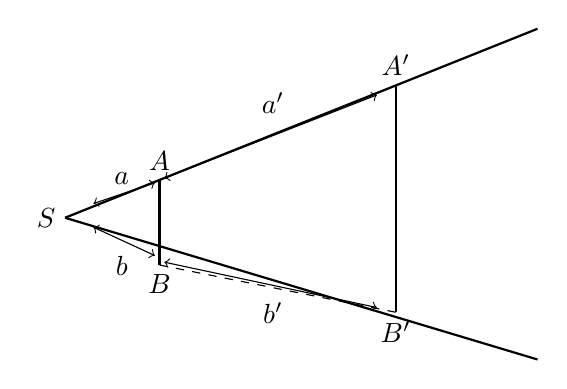
\begin{tikzpicture}[scale=1.2]
		% Rays
		\draw[thick] (0,0) -- (5,2); % upper ray
		\draw[thick] (0,0) -- (5,-1.5); % lower ray

		% Parallels
		\draw[thick] (1,0.4) -- (1,-0.5);
		\draw[thick] (3.5,1.4) -- (3.5,-1);

		% Points
		\node at (-0.2,0) {\(S\)};
		\node[above] at (1,0.4) {\(A\)};
		\node[below] at (1,-0.5) {\(B\)};
		\node[above] at (3.5,1.4) {\(A'\)};
		\node[below] at (3.5,-1) {\(B'\)};

		% Helper lines
		\draw[dashed] (1,0.4) -- (3.5,1.4);
		\draw[dashed] (1,-0.5) -- (3.5,-1);

		% Length labels
		\draw[<->] (0.3,0.15) -- (0.95,0.37);
		\node[above] at (0.6,0.25) {\(a\)};
		\draw[<->] (1.05,0.42) -- (3.3,1.3);
		\node[above] at (2.2,1) {\(a'\)};

		\draw[<->] (0.3,-0.1) -- (0.95,-0.4);
		\node[below] at (0.6,-0.3) {\(b\)};
		\draw[<->] (1.05,-0.47) -- (3.3,-0.95);
		\node[below] at (2.2,-0.8) {\(b'\)};
	\end{tikzpicture}
\end{center}

\subsubsection{Second Intercept Theorem (General Form)}

If a ray intersects two parallel lines, the segments from the origin point to the lines are in the same 
ratio as the segments along the parallels:

\[
	\frac{SA}{SA'} = \frac{SB}{SB'} \quad \text{and} \quad \frac{AB}{A'B'} = \frac{SA}{SA'}
\]

\begin{center}
	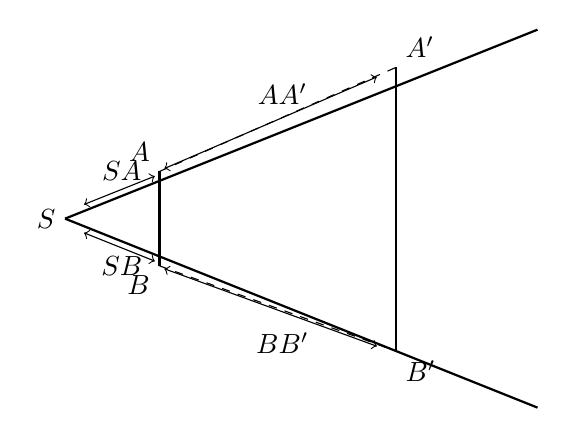
\begin{tikzpicture}[scale=1.2]
		% Rays
		\draw[thick] (0,0) -- (5,2); % upper ray
		\draw[thick] (0,0) -- (5,-2); % lower ray

		% Parallels
		\draw[thick] (1,0.5) -- (1,-0.5);
		\draw[thick] (3.5,1.6) -- (3.5,-1.4);

		% Points
		\node at (-0.2,0) {\(S\)};
		\node[above left] at (1,0.5) {\(A\)};
		\node[below left] at (1,-0.5) {\(B\)};
		\node[above right] at (3.5,1.6) {\(A'\)};
		\node[below right] at (3.5,-1.4) {\(B'\)};

		% Helper lines
		\draw[dashed] (1,0.5) -- (3.5,1.6);
		\draw[dashed] (1,-0.5) -- (3.5,-1.4);
		\draw[dashed] (1,0.5) -- (1,-0.5);
		\draw[dashed] (3.5,1.6) -- (3.5,-1.4);

		% Length labels
		\draw[<->] (0.2,0.15) -- (0.95,0.45);
		\node[above] at (0.6,0.3) {\(SA\)};
		\draw[<->] (1.05,0.53) -- (3.3,1.5);
		\node[above] at (2.3,1.1) {\(AA'\)};

		\draw[<->] (0.2,-0.15) -- (0.95,-0.45);
		\node[below] at (0.6,-0.3) {\(SB\)};
		\draw[<->] (1.05,-0.53) -- (3.3,-1.35);
		\node[below] at (2.3,-1.1) {\(BB'\)};
	\end{tikzpicture}
\end{center}

\subsection{Proof of the Pythagorean Theorem}

We want to prove that \(c^2 = a^2 + b^2\) is a true statement.

Let us a build a Square with area \(c^2\) and take our original triangle and put it on the sides
on the square.

This will create a square of sides \((a+b)^2\) which is bigger than the inner square \(c^2\).

Now let us find the area \(c^2\) using what we know about this shape.

\begin{align*}
	{(a + b)}^2 = 4(\frac{ab}{2}) + c^2\\
	{(a + b)}^2 = 2ab + c^2\\
	a^2 + 2ab + b^2 = 2ab + c^2\\
	a^2 + b^2 = c^2
\end{align*}

\QED

